\documentclass[ucs]{beamer}

%\usepackage[ngerman]{babel}
%\usepackage[latin1]{inputenc}

\usepackage[utf8x]{inputenc}
\usepackage[all]{xy}
\usepackage{hyperref}
\usepackage{algorithm2e}
\usepackage{tikz}
\usepackage{listings}
\usepackage{xcolor}
\usepackage[absolute,overlay]{textpos}
\usepackage{graphicx} % Required for the inclusion of images
\usepackage{amsmath} % Required for some math elements 
\usepackage{ae} % Uml. im PDF-Verzeichnis
%\makeatletter

% to change colors
\newcommand{\fillcol}{green!20}
\newcommand{\bordercol}{black}

\setbeamercovered{transparent} 
\mode<presentation>{
	  \useoutertheme[subsection=false]{miniframes}
	    \useinnertheme{rectangles}
		   \usecolortheme{crane}
}


\title{A Lattice Boltzmann Method for immiscible multiphase flow simulations using the Level Set Method} % Title

\author{Lorenz Hufnagel, Daniel Zint} % Author name
\institute{BGCE Student Project}

\date{x y, 2015} % Date for the report

\begin{document}

\maketitle % Insert the title, author and date

\section{Motivation \& Introduction}

\begin{frame}
\frametitle{Multiphase flow - Examples}
\begin{itemize}
\item<1-> Examples
\item<2-> e.g. Oil in water 
\item<3-> \ldots
\end{itemize}
\end{frame}

\section{Mathematic foundation}
\begin{frame}
\frametitle{Macroscopic fluid mechanics}

\begin{itemize}
\item<1-> $N$ immiscible fluids.
\item<2-> Each has own $\rho_i, \nu_i$
\item<3-> Hydrodynamics described by (incompressible) NSE
\end{itemize}
\visible<3->{
$$
\nabla \cdot  \vec v = 0
$$
$$
\frac{\partial \vec v}{\partial t} + \left(\vec  v \cdot \nabla \right) \vec v
=
-\frac{1}{\rho_i}\nabla p + \nu_i \nabla^2 \vec v $$
}
\end{frame}

\begin{frame}
\frametitle{Mathematic foundation}
\framesubtitle{Interface conditions}
\begin{figure}[h!]
    %\flushright
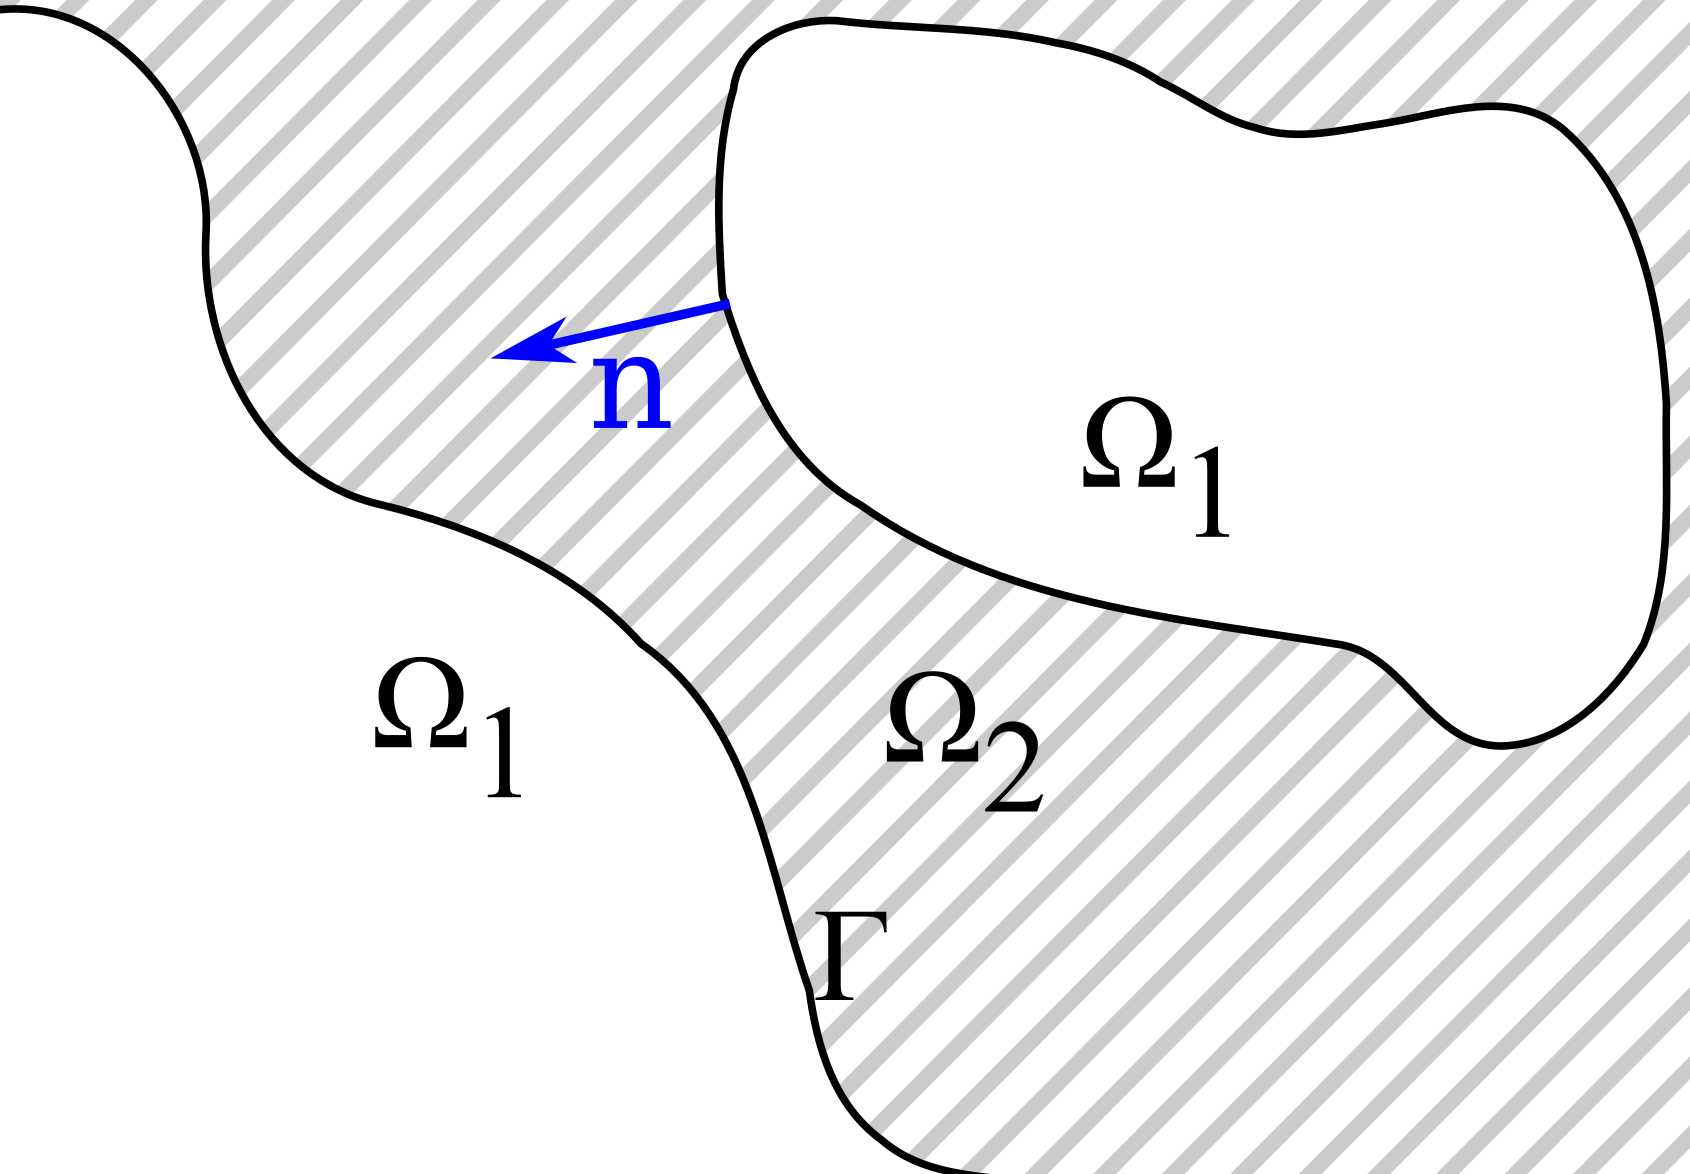
\includegraphics[width=6cm]{skizze.png}
  \caption{Two fluid domains $\Omega_i$ and interface $\Gamma$ inbetween}
\end{figure}
\begin{itemize}
\item<1-> Velocity across interface is $C_0$-continous 
  $$\lim_{\epsilon \to 0}(\vec v\left(x+\epsilon \vec n\right) -\vec v(x-\epsilon \vec n))=0$$
\end{itemize}
\end{frame}

\begin{frame}
\frametitle{Mathematic foundation}
\framesubtitle{Interface conditions cont'd}
\begin{figure}[h!]
    %\flushright
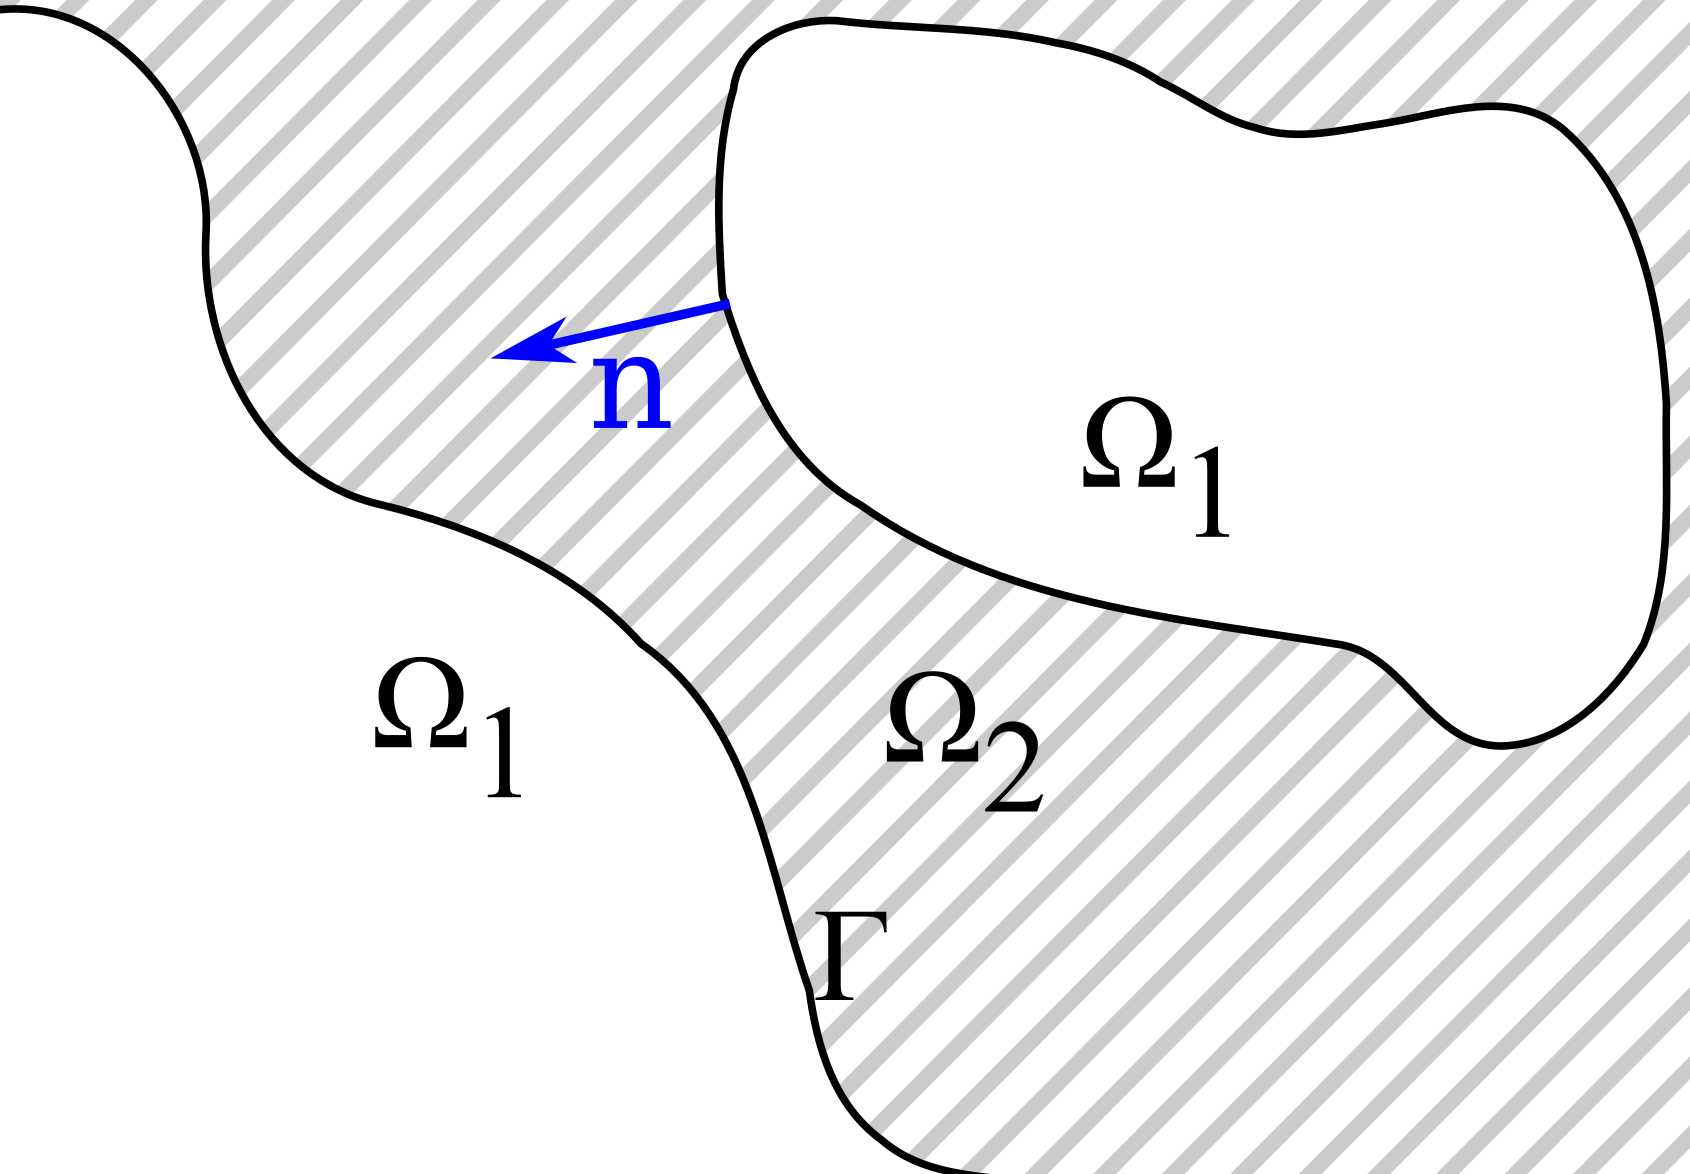
\includegraphics[width=4cm]{skizze.png}
  %\caption{Two fluid domains $\Omega_i$ and interface $\Gamma$ inbetween}
\end{figure}
\begin{itemize}
\item<1->Normal stress is balanced by surface tension
  $$\lim_{\epsilon \to 0}(\textbf{T}_2(x+\epsilon \vec n) - \textbf{T}_1(x-\epsilon \vec n)) \cdot \vec n= 2\sigma \kappa \vec n$$
\end{itemize}
\vspace{-.5cm}
\visible<2->{
  where $\textbf{T}_i$ is the stress tensor $\textbf{T}_i=2\nu_i \rho_i \textbf{S}_i -p \textbf{Id}$ and $\kappa$ is the curvature of the interface $\nabla \cdot \vec n$. $\textbf{S} = \frac{1}{2}(\partial_{x_i} v_j+\partial_{x_j}  v_i)$
}
\end{frame}

\begin{frame}
\frametitle{Mathematic foundation}
\framesubtitle{Interface capturing}
The interface between fluid phases is captured by a Level-Set Method.

I.e. a \textit{level set function} $\phi:= \phi(x,t) \rightarrow \mathbb{R}$ is tracked through the fluid domain. The interface is given by the zero-isosurface of this function.
It holds:
$$ \frac{\partial \phi}{\partial t} + \vec v \cdot \nabla \phi = 0.$$
%todo benefits erklaeren
\end{frame}

\begin{frame}
\frametitle{Mathematic foundation}
\framesubtitle{Interface capturing}
Level-Set function only stored in narrow band around interface, Adalsteinsson and Sethian
TODO: Quellen als Footnotes + Uebersichtsfolie

Interface properties (curvature, normal) are obtained from discrete level-set function by weighted least-squares method.
\end{frame}

\begin{frame}
\frametitle{Mathematic foundation}
\framesubtitle{Interface capturing}
Hydrodynamics are solved by LBM.

<Coupling und BC's erklären!!\ldots>
\end{frame}

\section{Results}
\begin{frame}
\frametitle{Validation}
\framesubtitle{Validation setups}
\end{frame}

\section{Outlook}
\begin{frame}
\frametitle{Conclusion \& Outlook}
$\rightarrow$ \dots

\vspace{.8cm}
Outlook:
\begin{itemize}
\item<1-> Include thermal flow (simulate e.g. lava lamp)
\item<2-> \dots
\end{itemize}

\end{frame}

\begin{frame}
\frametitle{References}
\begin{thebibliography}{etw}
   \bibitem{thoemmes}
     Thömmes, Guido, et al. "A lattice Boltzmann method for immiscible multiphase flow simulations using the level set method." Journal of Computational Physics 228.4 (2009): 1139-1156
\end{thebibliography}
\end{frame}

\end{document}
